\documentclass[11pt]{article}

%% PACKAGES
\usepackage{graphicx}
\usepackage[printonlyused]{acronym}
\usepackage{float}
\usepackage[colorlinks=false]{hyperref}
\usepackage{tabularx}
\usepackage{caption}
\usepackage[margin=1.0in]{geometry}
\usepackage{tocloft}
\usepackage{listings}

\lstset{basicstyle=\small\ttfamily,columns=flexible,breaklines=true,xleftmargin=0.5in,keepspaces=true}


\makeatletter
\g@addto@macro\normalsize{%
  \setlength\abovedisplayskip{0.25pt}
  \setlength\belowdisplayskip{0.25pt}
  \setlength\abovedisplayshortskip{0.25pt}
  \setlength\belowdisplayshortskip{0.25pt}
}
\makeatother

\setlength{\parskip}{\baselineskip}

%% GRAPHICS PATH
\graphicspath{{../../../shared_latex_inputs/images}{../../../shared_latex_inputs/graphs}}

\newcommand{\acposs}[1]{%
	\expandafter\ifx\csname AC@#1\endcsname\AC@used
	\acs{#1}'s%
	\else
	\aclu{#1}'s (\acs{#1}'s)%
	\fi
}

\title{\Huge EMTG Tutorial: Journey Boundaries}
\vspace{0.5cm}
\author
{
	Tim Sullivan \thanks{Aerospace Engineer, The Aerospace Corporation}
}
\vspace{0.5cm}

\newcommand{\listofknownissuesname}{\Large List of Known Issues}
\newlistof{knownissues}{mcf}{\listofknownissuesname}

\newcommand{\knownissue}[3]
{
	\refstepcounter{knownissues}
	\par\noindent\textbf{\hyperref[#2_b]{\theknownissues\quad #1}}\label{#2_h}
	\textbf{\hfill\pageref{#2_b}}
	#3
}

\newcommand{\knownissuelabel}[2]
{
	 \phantomsection
  	\hyperref[#2_h]{#1}\def\@currentlabel{\unexpanded{#1}}\label{#2_b}
}

\begin{document}

\begin{titlepage}
\maketitle
\thispagestyle{empty}
\begin{table}[H]
	\centering
	\begin{tabularx}{\textwidth}{|l|l|X|}
		\hline
		\textbf{Revision Date} & \textbf{Author} & \textbf{Description of Change} \\
		\hline
		\date{December 2, 2022} & Tim Sullivan & Initial revision.\\
		\hline
		\date{June 30, 2023} & Joseph Hauerstein & Conversion to \LaTeX.\\ 
		\hline
		\date{August 4, 2023} & Joseph Hauerstein & Addition of Known Issues section.\\ 
		\hline
	\end{tabularx}
\end{table}
\end{titlepage}

\newpage
\tableofcontents
\thispagestyle{empty}
\newpage

\listofknownissues
\thispagestyle{empty}

\newpage
\clearpage
\setcounter{page}{1}



\section*{List of Acronyms}
\begin{acronym}
%To define the acronym and include it in the list of acronyms: \acro{acronym}{definition}
%To define the acronym and exclude it from the list of acronyms:  \acro{acronym}{definition}
%
%\ac{acronym} Expand and identify the acronym the first time; use only the acronym thereafter
%\acf{acronym} Use the full name of the acronym.
%\{acronym} Use the acronym, even before the first corresponding \ac command
%\acl{acronym}  Expand the acronym without using the acronym itself.
%
%

\acro{ACS}{attitude control system}
\acro{ACO}{Ant Colony Optimization}
\acro{AD}{Automatic Differentiation}
\acro{ADL}{Architecture Design Laboratory}
\acro{AES}{Advanced Exploration Systems}
\acro{AGA}{aerogravity assist}
\acro{ALARA}{As Low As Reasonably Achievable}
\acro{API}{application programming interface}
\acro{BB}{branch and bound}
\acro{BVP}{Boundary Value Problem}
\acro{CATO}{Computer Algorithm for Trajectory Optimization}
\acro{CL}{confidence level}
\acro{CONOPS}{concept of operations}
\acro{COV}{Calculus of Variations}
\acro{D/AV}{Descent/Ascent Vehicle}
\acro{DE}{Differential Evolution}
\acro{DLA}{Declination of Launch Asymptote}
\acro{RLA}{Right Ascension of Launch Asymptote}
\acro{RA}{right ascension}
\acro{DEC}{declination}
\acro{DPTRAJ/ODP}{Double Precision Trajectory and Orbit Determination Program}
\acro{DSH}{Deep Space Habitat}
\acro{DSN}{Deep Space Network}
\acro{DSMPGA}{Dynamic-Size Multiple Population Genetic Algorithm}
\acro{EB}{Evolutionary Branching}
\acro{ECLSS}{environmental control and life support system}
\acro{ELV}{expendable launch vehicle}
\acro{EMME}{Earth to Mars, Mars to Earth}
\acro{EMMVE}{Earth to Mars, Mars to Venus to Earth}
\acro{EMTG}{Evolutionary Mission Trajectory Generator}
\acro{EVMME}{Earth to Venus to Mars, Mars to Earth}
\acro{EVMMVE}{Earth to Venus to Mars, Mars to Venus to Earth}
\acro{ERRV}{Earth Return Re-entry Vehicle}
\acro{FISO}{Future In-Space Operations}
\acro{FMT}{Fast Mars Transfer}
\acro{GASP}{Gravity Assist Space Pruning}
\acro{GCR}{galactic cosmic radiation}
\acro{GRASP}{Greedy Randomized Adaptive Search Procedure}
\acro{GSFC}{Goddard Space Flight Center}
\acro{GTOC}{Global Trajectory Optimization Competition}
\acro{GTOP}{Global Trajectory Optimization Problem}
\acro{HAT}{Human Architecture Team}
\acro{HGGA}{Hidden Genes Genetic Algorithm}
\acro{IMLEO}{Initial Mass in \acl{LEO}}
\acro{IPOPT}{Interior Point OPTimizer}
\acro{ISS}{International Space Station}
\acro{JHUAPL}{Johns Hopkins University Applied Physics Laboratory}
\acro{JSC}{Johnson Space Center}
\acro{KKT}{Karush-Kuhn-Tucker}
\acro{LEO}{Low Earth Orbit}
\acro{LRTS}{lazy race tree search}
\acro{MONTE}{Mission analysis, Operations, and Navigation Toolkit Environment}
\acro{MCTS}{Monte Carlo tree search}
\acro{MGA}{Multiple Gravity Assist}
\acro{MIRAGE}{Multiple Interferometric Ranging Analysis using GPS Ensemble}
\acro{MOGA}{Multi-Objective Genetic Algorithm}
\acro{MOSES}{Multiple Orbit Satellite Encounter Software}
\acro{MPI}{message passing interface}
\acro{MPLM}{Multi-Purpose Logistics Module}
\acro{MSFC}{Marshall Space Flight Center}
\acro{NELLS}{NASA Exhaustive Lambert Lattice Search}
\acro{NSGA}{Non-Dominated Sorting Genetic Algorithm}
\acro{NSGA-II}{Non-Dominated Sorting Genetic Algorithm II}
\acro{NHATS}{Near-Earth Object Human Space Flight Accessible Targets Study}
\acro{NTP}{Nuclear Thermal Propulsion}
\acro{OD}{orbit determination}
\acro{OOS}{On-Orbit Staging}
\acro{PCC}{Pork Chop Contour}
\acro{PEL}{permissible exposure limits}
\acro{PLATO}{PLAnetary Trajectory Optimization}
\acro{REID}{risk of exposure-induced death}
\acro{RTBP}{Restricted Three Body Problem}
\acro{SA}{Simulated Annealing}
\acro{SLS}{Space Launch System}
\acro{SNOPT}{Sparse Nonlinear OPTimizer}
\acro{SOI}{sphere of influence}
\acro{SPE}{solar particle events}
\acro{SQP}{sequential quadratic programming}
\acro{SRAG}{Space Radiation Analysis Group}
\acro{TEI}{Trans-Earth Injection}
\acro{TOF}{time of flight}
\acro{TPBVP}{Two Point Boundary Value Problem}
\acro{TMI}{Trans-Mars Injection}
\acro{VARITOP}{Variational calculus Trajectory Optimization Program}
\acro{VILM}{v-infinity leveraging maneuver}
\acro{MOI}{Mar Orbit Injection}
\acro{PCM}{Pressurized Cargo Module}
\acro{STS}{Space Transportation System}
\acro{EDS}{Earth Departure Stage}
\acro{NEO}{near-Earth asteroid}
\acro{IDC}{Integrated Design Center}
\acro{SEP}{solar-electric propulsion}
\acro{SRP}{solar radiation pressure}
\acro{NEP}{nuclear-electric propulsion}
\acro{REP}{radioisotope-electric propulsion}
\acro{DRM}{Design Reference Missions}

\acro{EDL}{entry, descent, and landing}
\acro{ASCII}{American Standard Code for Information Interchange}
\acro{AU}{Astronomical Unit}
\acro{BWG}{Beam Waveguides}
\acro{CCB}{Configuration Control Board}
\acro{CMO}{Configuration Management Office}
\acro{CODATA}{Committee on Data for Science and Technology}
\acro{DEEVE}{Dynamically Equivalent Equal Volume Ellipsoid}
\acro{DRA}{Design Reference Asteroid}
\acro{EME2000}{Earth Centered, Earth Mean Equator and Equinox of J2000 (Coordinate Frame)}
\acro{EOP}{Earth Orientation Parameters}
\acro{ET}{Ephemeris Time}
\acro{FDS}{Flight Dynamics System}
\acro{FTP}{File Transfer Protocol}
\acro{GSFC}{Goddard Space Flight Center}
\acro{PI}{Principal Investigator}
\acro{HEF}{High Efficiency}
\acro{IAG}{International Association of Geodesy}
\acro{IAU}{International Astronomical Union}
\acro{IERS}{International Earth Rotation and Reference Systems Service}
\acro{ICRF}{International Celestial Reference Frame}
\acro{ITRF}{International Terrestrial Reference System}
\acro{IOM}{Interoffice Memorandum}
\acro{JD}{Julian Date}
\acro{JPL}{Jet Propulsion Laboratory}
\acro{LM}{Lockheed Martin}
%\acro{LP150Q}{}
%\acros{LP100K}{}
\acro{MAVEN}{Mars Atmosphere and Volatile EvolutioN}
\acro{MJD}{Modified Julian Date}
\acro{MOID}{Minimum Orbit Intersection Distance}
\acro{MPC}{Minor Planet Center}
\acro{NASA}{National Aeronautics and Space Administration}
\acro{NDOSL}{\ac{NASA} Directory of Station Locations}
\acro{NEA}{near-Earth asteroid}
\acro{NEO}{near-Earth object}
\acro{NIO}{Nav IO}
\acro{OSIRIS-REx}{Origins Spectral Interpretation Resource Identification Security-Regolith Explorer}
\acro{PHA}{Potentially Hazardous Asteroid}
\acro{PHO}{Potentially Hazardous Object}
\acro{SBDB}{Small-Body Database}
\acro{SI}{International System of Units}
\acro{SPICE}{Spacecraft Planet Instrument Camera-matrix Events}
\acro{SPK}{SPICE Kernel}
\acro{SRC}{Sample Return Capsule}
\acro{SSD}{Solar System Dynamics}
\acro{STK}{Systems Tool Kit}
\acro{TAI}{International Atomic Time}
\acro{TBD}{To Be Determined}
\acro{TBR}{To Be Reviewed}
\acro{TCB}{Barycentric Coordinate Time}
\acro{TDB}{Temps Dynamiques Barycentrique, Barycentric Dynamical Time}
\acro{TDT}{Terrestrial Dynamical Time}
\acro{TT}{Terrestrial Time}
\acro{URL}{Uniform Resource Locator}
\acro{UT}{Universal Time}
\acro{UT1}{Universal Time Corrected for Polar Motion}
\acro{UTC}{Coordinated Universal Time}
\acro{USNO}{U. S. Naval Observatory}
\acro{YORP}{Yarkovsky-O'Keefe-Radzievskii-Paddack}

\acro{NLP}{nonlinear program}
\acro{MBH}{monotonic basin hopping}
\acro{MBH-C}{monotonic basin hopping with Cauchy hops}
\acro{FBS}{forward-backward shooting}
\acro{MGALT}{Multiple Gravity Assist with Low-Thrust}
\acro{MGALTS}{Multiple Gravity Assist with Low-Thrust using the Sundman transformation}
\acro{MGA-1DSM}{Multiple Gravity Assist with One Deep Space Maneuver}
\acro{MGAnDSMs}{Multiple Gravity Assist with \textit{n} Deep-Space Maneuvers using Shooting}
\acro{PSFB}{Parallel Shooting with Finite-Burn}
\acro{PSBI}{Parallel Shooting with Bounded Impulses}
\acro{FBLT}{Finite-Burn Low-Thrust}
\acro{FBLTS}{Finite-Burn Low-Thrust using the Sundman transformation}
\acro{ESA}{European Space Agency}
\acro{ACT}{Advanced Concepts Team}
\acro{IRAD}{independent research and development}
\acro{Isp}[$\text{I}_{sp}$]{specific impulse}
\acro{C3}[$C_3$]{hyperbolic excess energy}
\acro{GA}{genetic algorithm}
\acro{GALLOP}{ Gravity Assisted Low-thrust Local Optimization Program}
\acro{MALTO}{Mission Analysis Low-Thrust Optimization}
\acro{PaGMO}{Parallel Global Multiobjective Optimizer}
\acro{FRA}{feasible region analysis}
\acro{CP}{conditional penalty}
\acro{HOC}{hybrid optimal control}
\acro{HOCP}{hybrid optimal control problem}
\acro{PSO}{particle swarm optimization}
\acro{SEPTOP}{Solar Electric Propulsion Trajectory Optimization Program}
\acro{STOUR}{Satellite Tour Design Program}
\acro{STOUR-LTGA}{Satellite Tour Design Program - Low Thrust, Gravity Assist}
\acro{PaGMO}{Parallel Global Multiobjective Optimizer}
\acro{SDC}{static/dynamic control}
\acro{DDP}{Differential Dynamic Programming}
\acro{HDDP}{Hybrid Differential Dynamic Programming}
\acro{ACT}{Advanced Concepts Team}
\acro{GMAT}{General Mission Analysis Toolkit}
\acro{BOL}{beginning of life}
\acro{EOL}{end of life}
\acro{KSC}{Kennedy Space Center}
\acro{VSI}{variable \ac{Isp}}
\acro{RTG}{radioisotope thermal generator}
\acro{ASRG}{advanced Stirling radiosotope generator}
\acro{ARRM}{Asteroid Robotic Redirect Mission}
\acro{AATS}{Alternative Architecture Trade Study}
\acro{PPU}{power processing unit}
\acro{STM}{state transition matrix}
\acro{MTM}{maneuver transition matrix}
\acro{HPTM}{half-phase transition matrix}
\acro{BCI}{body-centered inertial}
\acro{BCF}{body-centered fixed}
\acro{UTTR}{Utah Test and Training Range}
\acro{EPV}{equatorial projection of $\mathbf{v}_\infty$}
\acro{KBO}{Kuiper belt object}
\acro{DSM}{deep-space maneuver}
\acro{BPT}{body-probe-thrust}
\acro{4PL}{four parameter logistic}
\acro{BCF}{body-centered fixed}
\acro{COE}{classical orbit elements}
\acro{GSL}{Gnu Scientific Library}
\acro{NEXT}{NASA's Evolutionary Xenon Thruster}

\acro{SMA}{semi-major axis}
\acro{ECC}{eccentricity}

\acro{GSAD}{Ghosh Sparse Algorithmic Differentiation}

\end{acronym}

% --------------------------------------------------------------------------------------------------------------------------
% --------------------------------------------------------------------------------------------------------------------------


%%%%%%%%%%%%%%%%%%%%%
\section{Introduction}
\label{sec:introduction}
%%%%%%%%%%%%%%%%%%%%%

This tutorial assumes you have already completed the OSIRIS-REx and LowSIRIS-REx tutorials. While this tutorial doesn’t make use of the \ac{EMTG} files created in those tutorials, \ac{EMTG} options and features covered in past tutorials may not be covered in follow-on tutorials.

\noindent As you saw in the OSIRIS-REx tutorials, a typical \ac{EMTG} workflow is to begin with a low-fidelity solution and use that solution as the initial guess for higher fidelity models. This tutorial will walk you through creating another \ac{EMTG} options file for a mission launching from Earth, flying past Venus, and arriving at Mars using a patched conics solution. This is called the EVM (Earth-Venus-Mars) scenario. Then you will begin the process of making the mission increasingly realistic by defining specific departure and arrival state parameters. Follow-on tutorials will increase the realism of this and the OSIRIS-REx examples by adding additional forces and more accurate flybys.


%%%%%%%%%%%%%%%%%%%%%
\subsection{Patched Conics}
\label{sec:patched_conics}
%%%%%%%%%%%%%%%%%%%%%

The method of patched conics approximates interplanetary trajectories in a way that is useful for generating low-fidelity initial guesses for a mission. Patched conics takes a series of conic sections and connects them together between destinations in the solar system. Each conic section is a segment of an orbit around the central body, the Sun in this case. 

\noindent For example, in the EVM scenario, \ac{EMTG} attempts to find an ellipse with the Sun at one foci which connects Earth at the launch epoch to Venus at the flyby epoch and another ellipse connecting Venus to Mars at the arrival epoch. These are segments of different orbits around the Sun. Figure \ref{fig:patched_conic_ex} shows an example \ac{EMTG} solution from this tutorial. Shown in a red, dashed ellipse is the solar orbit connecting Venus and Mars which forms part of the patched conic solution. 

\noindent Notice that there is a \ac{DSM} between Earth and Venus. The trajectory from Earth to Venus is not a purely ballistic patched conic solution! Instead, there is a conic section defining the trajectory from Earth to the \ac{DSM} and another from the \ac{DSM} to Venus.

\begin{figure}[H]
	\centering
	\fbox{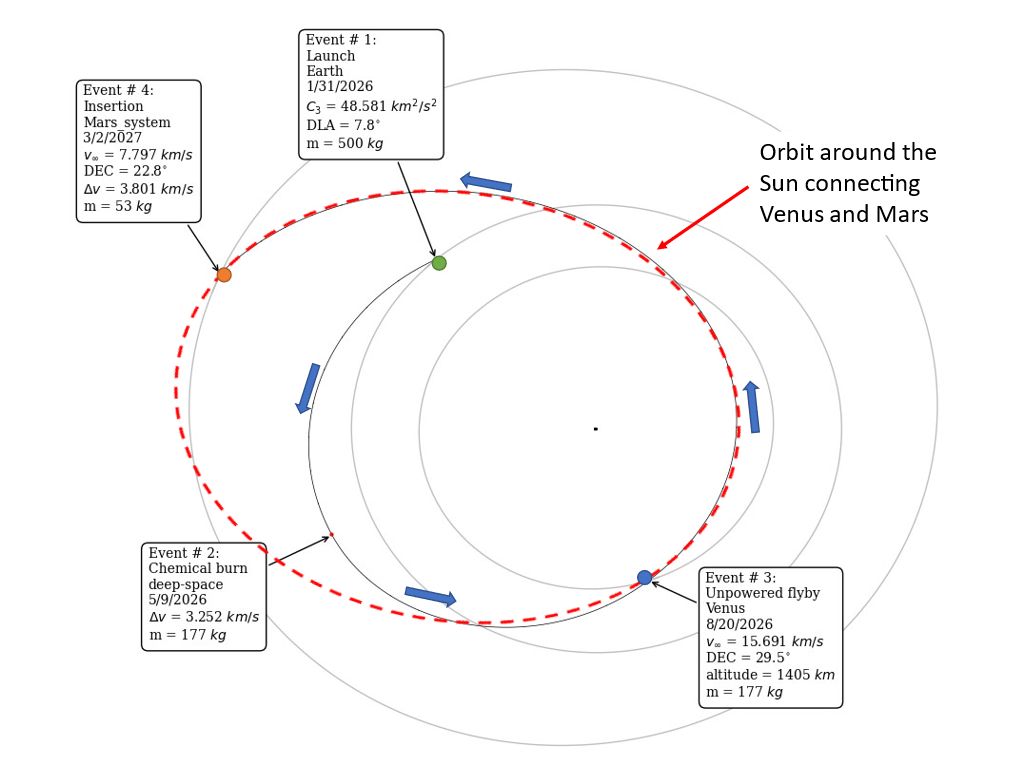
\includegraphics[width=\linewidth]{Journey_Boundaries_patched_conic_example.png}}
	\caption{\label{fig:patched_conic_ex}EVM MGAnDSM Patch Conic Example.}
\end{figure}

\noindent Patched conics are a good starting approximation because the gravitational forces exerted on the spacecraft are primarily due to the Sun and can be initially modeled by two-body forces. However, this is not accurate enough for realistic mission analysis. When the spacecraft is close to a planet, it is predominantly affected by the gravity of that planet rather than the Sun. The point where the transition between being predominantly affected by the planet’s gravity to predominantly affected by the Sun’s is called the \ac{SOI}. The approximate radius of the \ac{SOI} for a body is given by the equation below, where m is the mass of the smaller body, M is the mass of the larger body, and a is the semi-major axis of the smaller body’s orbit around the larger body.

\[ r_{SOI} \approx a(\frac{m}{M})^{2/5} \]

\noindent Additionally, as the spacecraft travels from one body to another, the gravitational forces of multiple bodies influence it. For example, a trajectory from Earth to Venus is affected by Jupiter’s gravity. You will add these perturbing gravitational forces and others in the non-two-body force model tutorial. 

\noindent Patched conics are also not a good high-fidelity solution because the conic sections begin and end at the center of mass of each body. For example, the Earth-to-Venus trajectory starts at Earth’s center of mass and ends at Venus’s center of mass. Obviously, you do not want the spacecraft to crash into a planet! These and other factors mean that the patched conic solution must be updated in order to fly the mission.

\noindent Up to this point, the \ac{EMTG} missions have used a patched conics approach to specify trajectory leg initial and final points. In this tutorial, the initial step will begin by making the missions more realistic by specifying trajectory leg end points that do not occur at the center of mass of an ephemeris object (i.e., a planet). The next tutorials will continue towards higher fidelity solutions by adding additional perturbing forces and more realistic body flybys.


%%%%%%%%%%%%%%%%%%%%%
\section{Setup}
\label{sec:setup}
%%%%%%%%%%%%%%%%%%%%%

Let’s create the patched conic Earth-Venus-Mars trajectory. This will be the basis for finding an initial solution and then migrating to higher fidelity.

%%%%%%%%%%%%%%%%%%%%%
\subsection{Global Options}
\label{sec:global_options}
%%%%%%%%%%%%%%%%%%%%%

Begin by creating the mission and Universe directory structure discussed in the introductory tutorial. For the EVM series of tutorials, you will only need the default ephemeris files \texttt{DE430.bsp}, \texttt{naif0012.tls}, and \texttt{pck00010.tpc}. Use the \ac{EMTG} universe file \texttt{Sun.emtg\_universe}, which is available from the tutorial documents in \texttt{docs/0\_Users/tutorial/Tutorial\_EMTG\_Files/EVM\_univ erse}. Place these files into an \texttt{EVM\_universe} directory using the structure shown in Figure \ref{fig:mission_dir_structure}. Similarly, the contents of \texttt{hardware\_models} are in Tutorial\_EMTG\_Files under \texttt{Journey\_Boundaries/ha rdware\_models}.

\begin{figure}[H]
	\centering
	\fbox{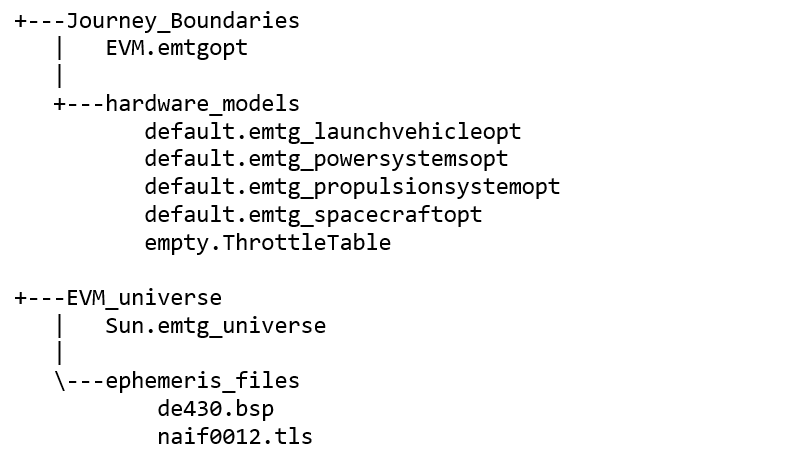
\includegraphics[width=0.8\linewidth]{Journey_Boundaries_mission_directory_structure.png}}
	\caption{\label{fig:mission_dir_structure}Mission Directory Structure.}
\end{figure}

\noindent Start PyEMTG and create a new mission (File-\textgreater New-\textgreater Mission or Ctrl+m). Set the following global options as shown in Figure \ref{fig:global_options}:

\begin{itemize}
	\item \textbf{Mission name:} ``EVM''
	\begin{itemize}
		\item Make sure to save the options file.
	\end{itemize}
	\item \textbf{Mission type:} ``\acs{MGAnDSMs}''
	\item \textbf{Objective function:} ``0 - minimum deterministic deltaV''
	\item \textbf{Launch window open date:} ``1 January 2026'' or ``61041.0''
	\item \textbf{Enable mission time bounds:} ``On''
	\item \textbf{Global flight time bounds:} ``0.0" to ``395.25'' days
	\item \textbf{Forced post-launch coast duration:} ``15'' days
	\item \textbf{Forced pre-flyby coast duration:} ``30'' days
	\item \textbf{forced post-flyby coast duration:} ``15'' days
\end{itemize}

\begin{figure}[H]
	\centering
	\fbox{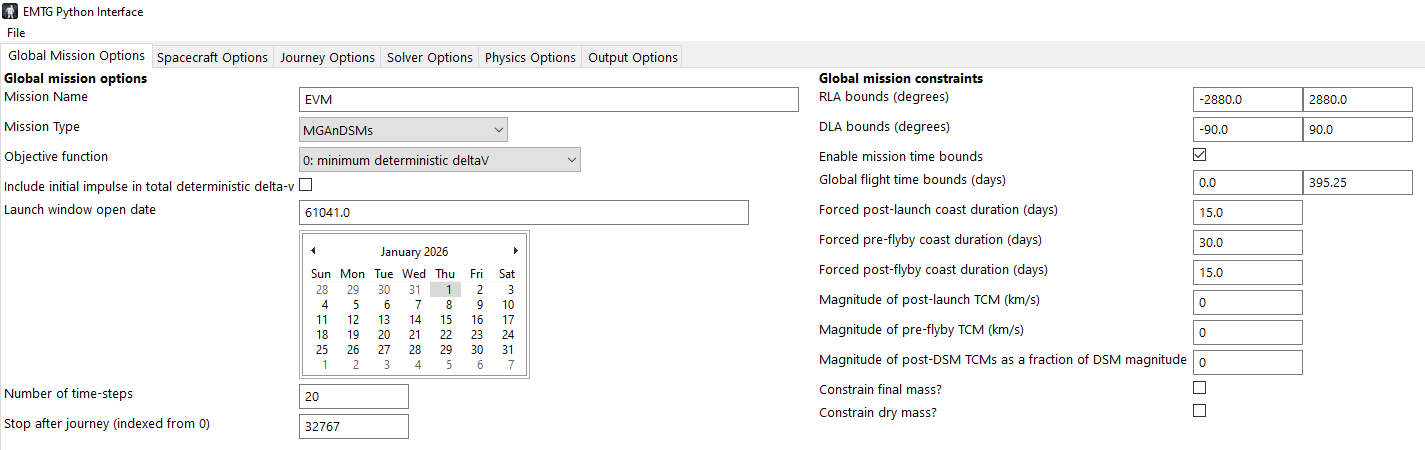
\includegraphics[width=\linewidth]{Journey_Boundaries_global_options.png}}
	\caption{\label{fig:global_options}EVM Global Options.}
\end{figure}

%%%%%%%%%%%%%%%%%%%%%
\subsection{Spacecraft Options}
\label{sec:spacecraft_options}
%%%%%%%%%%%%%%%%%%%%%

Select the ``Spacecraft Options'' tab and make the following changes as shown in Figure \ref{fig:spacecraft_options}:

\begin{itemize}
	\item \textbf{Maximum mass:} ``500'' kg
	\item \textbf{Spacecraft model type:} ``Assemble from missionoptions object''
	\item \textbf{Hardware library path:} path to ``\texttt{hardware\_models}''
	\begin{itemize}
		\item Do not forget the trailing slash.
	\end{itemize}
	\item \textbf{Launch vehicle library file:} ``\texttt{default.emtg\_launchvehicleopt}''
	\item \textbf{Launch vehicle:} ``ExampleRocket''
	\item \textbf{Chemical Isp:} ``320'' seconds
	\begin{itemize}
		\item Chemical Isp is used for \ac{DSM}s and assumes a bipropellant thruster.
	\end{itemize}
	\item \textbf{TCM Isp:} ``200'' seconds
	\begin{itemize}
		\item TCM Isp is used for pre/post event TCMs and Journey-end delta-v and TCMs. Assumed to be a monopropellant thruster.
	\end{itemize}
\end{itemize}

\begin{figure}[H]
	\centering
	\fbox{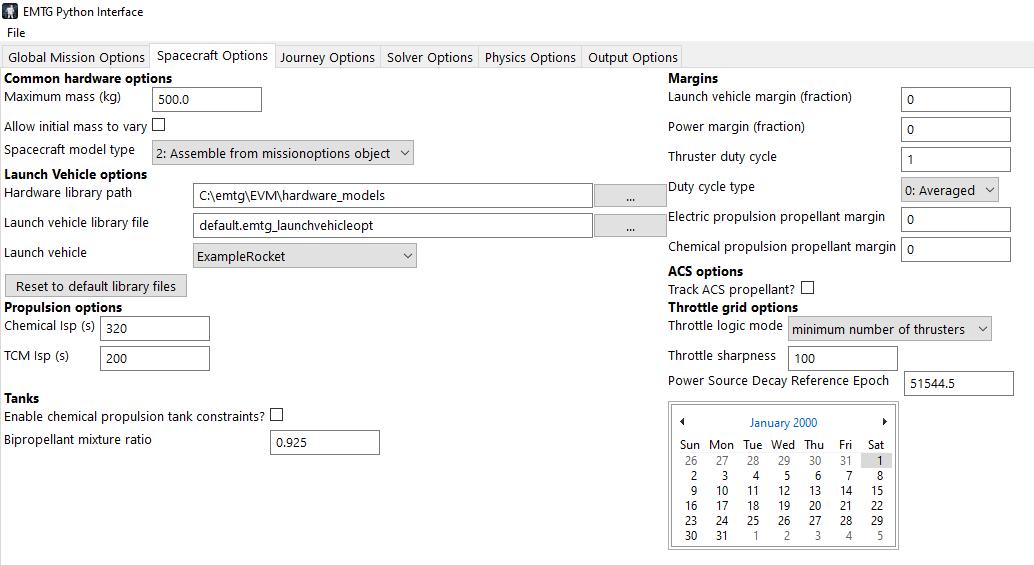
\includegraphics[width=\linewidth]{Journey_Boundaries_spacecraft_options.png}}
	\caption{\label{fig:spacecraft_options}EVM Spacecraft Options.}
\end{figure}

%%%%%%%%%%%%%%%%%%%%%
\subsection{Journey Options}
\label{sec:journey_options}
%%%%%%%%%%%%%%%%%%%%%

Select the ``Journey Options'' tab. You will create one Journey beginning at Earth, flying past Venus, and ending at Mars. Make the following changes to the default Journey as shown in Figure \ref{fig:journey_options}:

\begin{itemize}
	\item \textbf{Central body:} ``\texttt{Sun.emtg\_universe}''
	\begin{itemize}
		\item If \texttt{Sun.emtg\_universe} does not appear as an option for the central body, the most likely cause is that the default universe folder was not set to the folder that contains \texttt{Sun.emtg\_universe}. To override the default, select the ``Physics Options'' tab, and change the value of the ``Universe folder'' to the folder that contains \texttt{Sun.emtg\_universe}. Then, return to the ``Journey Options'' tab.
	\end{itemize}
	\item \textbf{Start location:} ``3'' for Earth
	\item \textbf{Final location:} ``4'' for Mars\_system
	\item \textbf{Wait time bounds:} ``0'' to ``30'' days
	\begin{itemize}
		\item Set the launch window open date in the ``Global Options'' tab to 1 January 2026. Setting 30 days as the upper bound here means that \ac{EMTG}’s solutions must depart Earth by 31 January 2026. If that sounds overly constrained, it is. You will find a better time to launch in a later tutorial.
	\end{itemize}
	\item \textbf{Journey time bounds:} ``bounded flight time''
	\item \textbf{Journey flight time bounds:} ``0'' to ``395.25''
	\begin{itemize}
		\item This means the solution has up to 13 months to arrive at Mars.
	\end{itemize}
	\item \textbf{Journey inital impulse boudns:} ``0'' to ``6.97'' km/s
	\item \textbf{Journey departure type:} ``0: launch or direct insertion''
	\item \textbf{Journey departure class:} ``0: Ephemeris-pegged''
	\item \textbf{Forced initial coast:} ``0'' days
	\item \textbf{Journey arrival type:} ``0: insertion into parking orbit (use chemical Isp)''
	\item \textbf{Journey arrival class:} ``0: Ephemeris-pegged''
	\item \textbf{Insertion orbit SMA:} ``20000'' km
	\item \textbf{Insertion orbit ECC:} ``0.7''
	\item \textbf{Forced terminal coast:} ``15'' days
	\item \textbf{Flyby sequence:} ``[2]''
	\begin{itemize}
		\item Venus is body \#2 in the Universe file.
	\end{itemize}
\end{itemize}

\begin{figure}[H]
	\centering
	\fbox{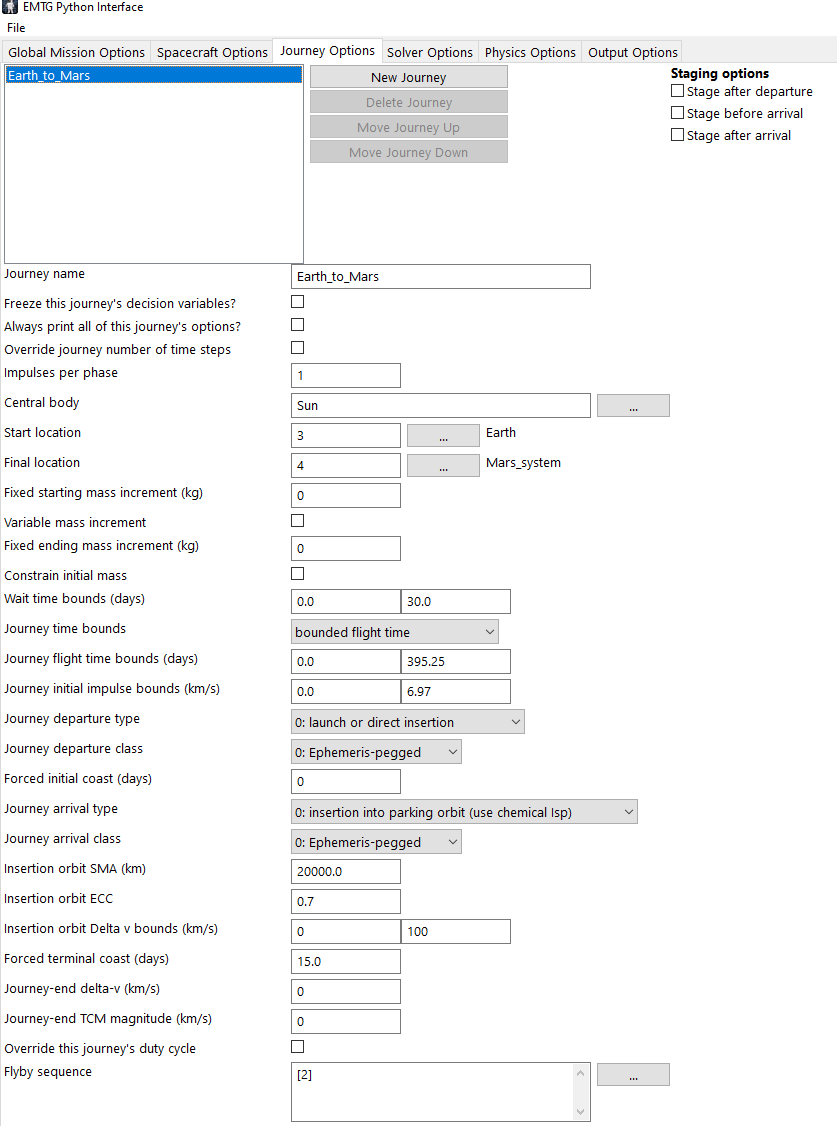
\includegraphics[width=\linewidth]{Journey_Boundaries_journey_options.png}}
	\caption{\label{fig:journey_options}EVM Journey Options.}
\end{figure}

%%%%%%%%%%%%%%%%%%%%%
\subsection{Solver Options}
\label{sec:solver_options}
%%%%%%%%%%%%%%%%%%%%%

Switch to the “Solver Options” tab. Most of these can remain set to their defaults, but it is recommended to change the following settings as shown in Figure \ref{fig:solver_options}:

\begin{itemize}
	\item \textbf{\acs{NLP} Chaperone:} ``On''
	\item \textbf{ACE feasible point finder:} ``On''
	\item \textbf{Maximum run-time(s):} ``120'' seconds
\end{itemize}

\begin{figure}[H]
	\centering
	\fbox{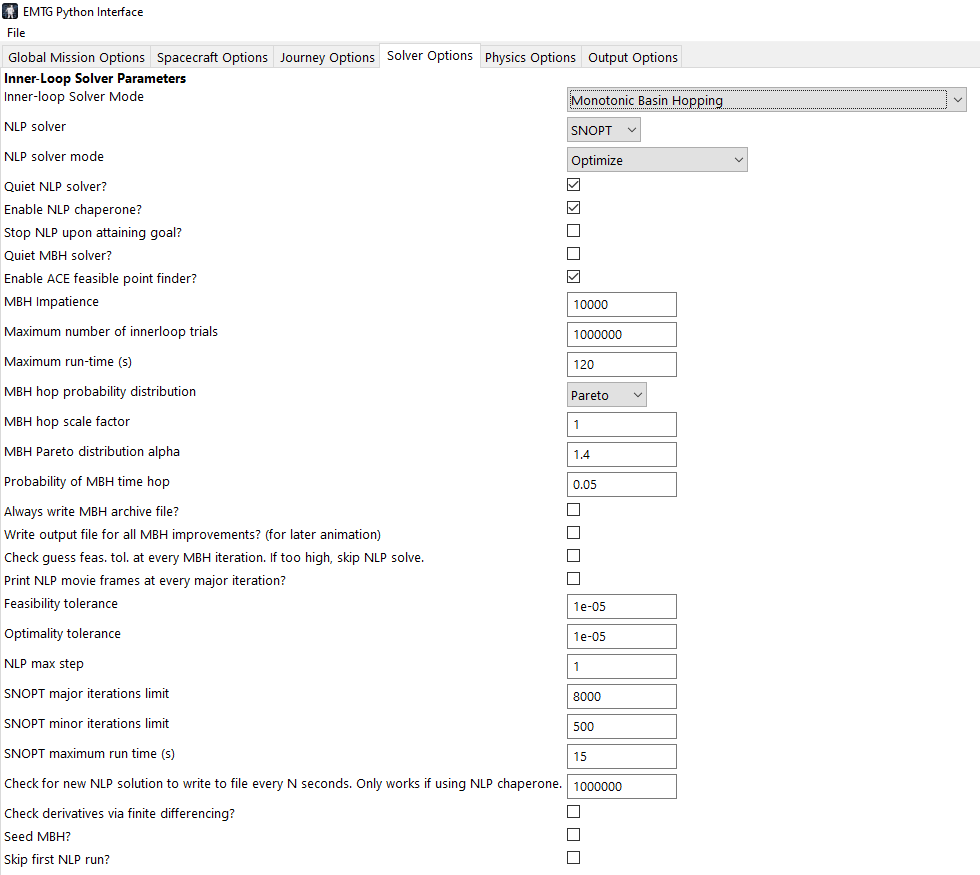
\includegraphics[width=\linewidth]{Journey_Boundaries_solver_options.png}}
	\caption{\label{fig:solver_options}EVM Solver Options.}
\end{figure}

%%%%%%%%%%%%%%%%%%%%%
\subsection{Physics Options}
\label{sec:ohysics_options}
%%%%%%%%%%%%%%%%%%%%%

Switch to the ``Physics Options'' tab. Because you’re just using the DE430 ephemeris, leave the earliest and latest spline epochs as their default value. Make sure to change the Universe folder path if you haven’t already. \ac{EMTG} will look in the path specified by ``Physics Options'' for the central bodies set in the Journey tab. If \ac{EMTG} can’t find them, it will throw an error at runtime. Even if you change the path to the central body Universe file in ``Journey Options'', \ac{EMTG} will look for a Universe file with that central body name inside the directory specified by ``Physics Options'', not the one you set in ``Journey Options''. Make sure to update this path whenever copying missions. The recommended settings are shown in Figure \ref{fig:physics_options}, but they should already be set.

\begin{figure}[H]
	\centering
	\fbox{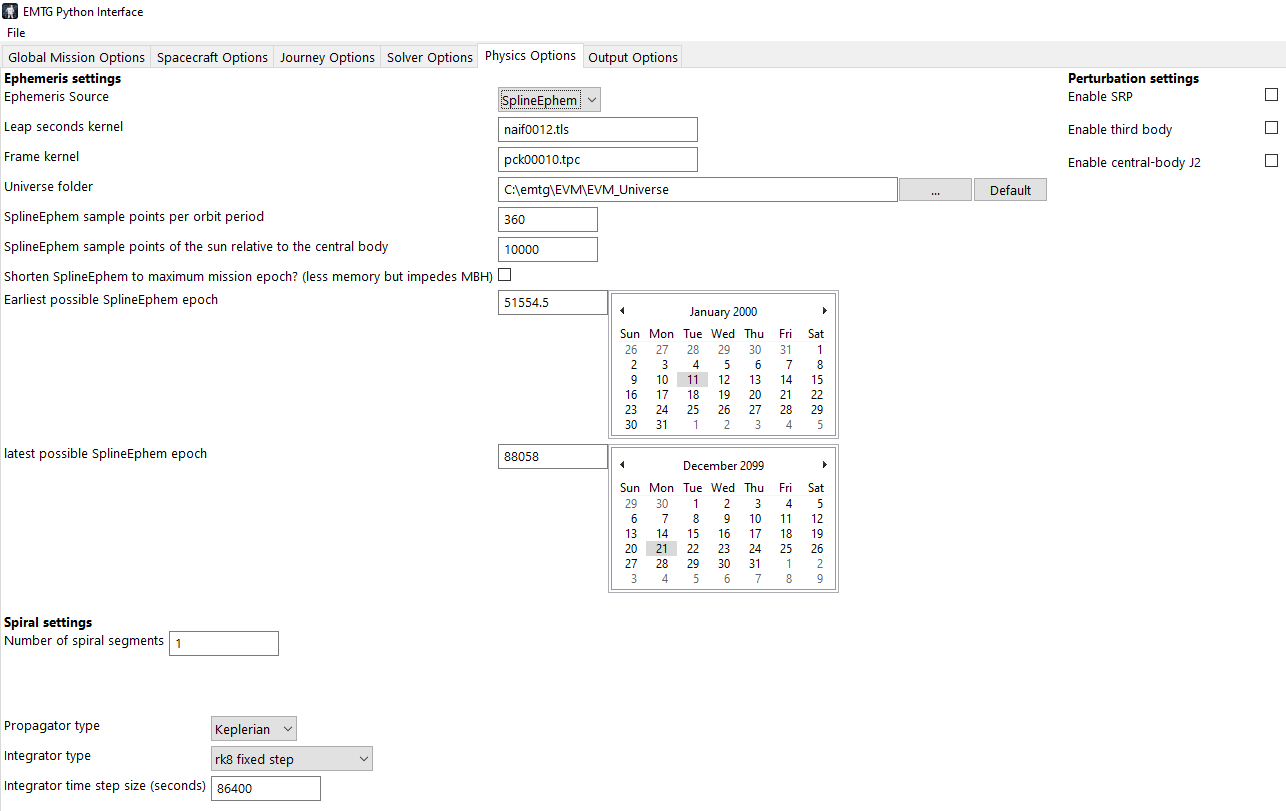
\includegraphics[width=\linewidth]{Journey_Boundaries_physics_options.png}}
	\caption{\label{fig:physics_options}EVM Physics Options.}
\end{figure}

%%%%%%%%%%%%%%%%%%%%%
\subsection{Output Options}
\label{sec:output_options}
%%%%%%%%%%%%%%%%%%%%%

Following the method used in the OSRIS-REx tutorial, create a \texttt{results} folder in the mission directory to hold the \ac{EMTG} outputs from each run. Switch to the ``Output Options'' tab and make the following changes as shown in Figure \ref{fig:output_options}:

\begin{itemize}
	\item \textbf{Output file frame:} ``\acs{ICRF}''
	\item \textbf{Override working directory:} ``On''
	\item \textbf{Working directory:} path to the \texttt{results} directory
\end{itemize}

\begin{figure}[H]
	\centering
	\fbox{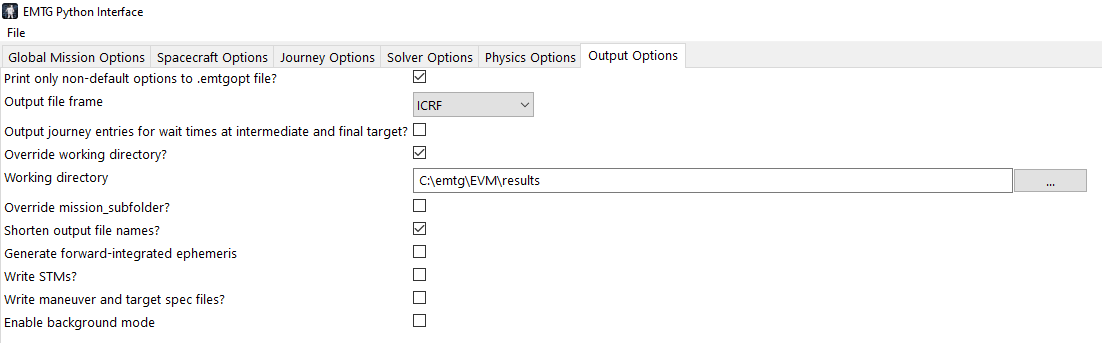
\includegraphics[width=\linewidth]{Journey_Boundaries_output_options.png}}
	\caption{\label{fig:output_options}EVM Output Options.}
\end{figure}

%%%%%%%%%%%%%%%%%%%%%
\section{Run and Post-Process}
\label{sec:run_and_post_process}
%%%%%%%%%%%%%%%%%%%%%

Select ``File-\textgreater Run'' (Ctrl+r), saving the file as \texttt{EVM.emtgopt}. After \ac{EMTG} finishes running, open the solution \texttt{EVM.emtg} file with PyEMTG (``File-\textgreater Open'', or Ctrl+o) and plot the trajectory. This is the patched conic solution. Note that your trajectory may look different than Figure \ref{fig:patched_conic_traj} because \ac{EMTG} uses stochastic optimization techniques and you only let \ac{EMTG} run 2 minutes. Next, you’ll modify the mission to have a more realistic arrival at Mars.

\begin{figure}[H]
	\centering
	\fbox{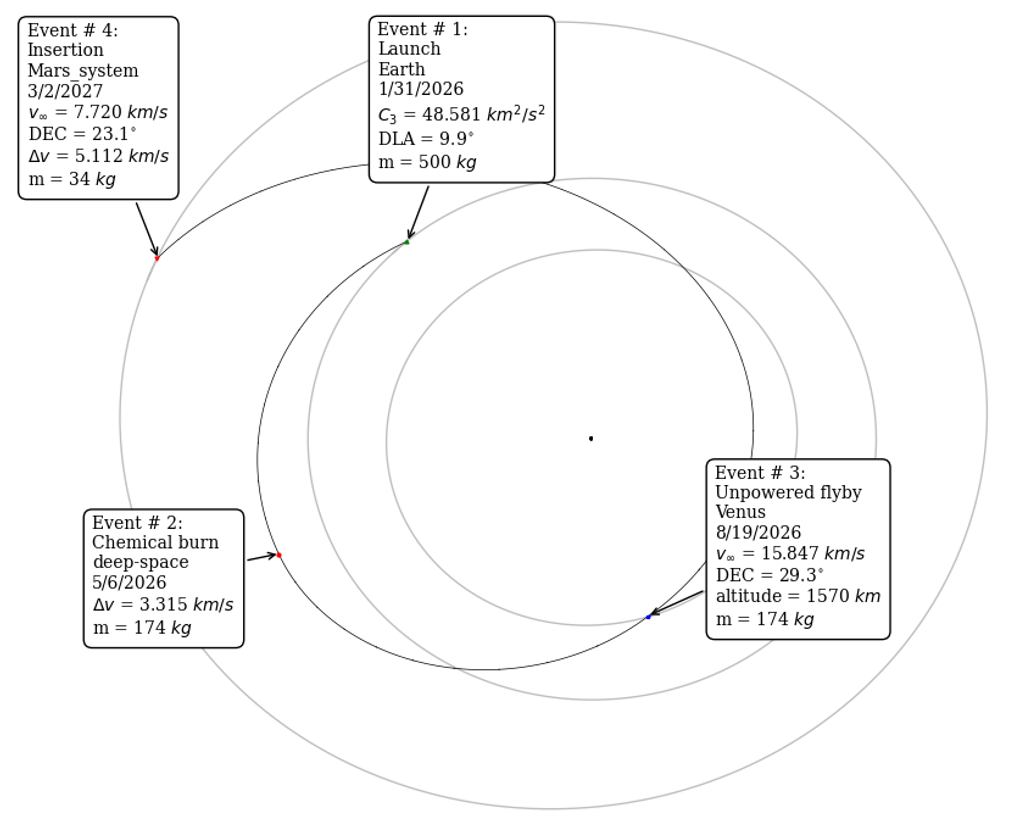
\includegraphics[width=0.65\linewidth]{Journey_Boundaries_EVM_patched_conic_trajectory.png}}
	\caption{\label{fig:patched_conic_traj}Earth Venus Mars Patched Conic Trajectory.}
\end{figure}

%%%%%%%%%%%%%%%%%%%%%
\section{Journey Boundaries}
\label{sec:journey_boundaries}
%%%%%%%%%%%%%%%%%%%%%

In \ac{EMTG}, a Boundary State defines the state of the spacecraft at the start (departure) or end (arrival) of a trajectory segment, such as a Phase or a Journey. Examples include the initial departure state from Earth or rendezvous with another body. Boundaries can be defined in several ways, and these definitions can be used to progress a solution from initial low-fidelity models to high-fidelity models.

\noindent In general, a user has much more flexibility in defining a \textit{Journey} Boundary than in defining a \textit{Phase} Boundary, and the remainder of this discussion is focused on Journey Boundaries.

%%%%%%%%%%%%%%%%%%%%%
\subsection{Ephemeris-Pegged Boundary Class}
\label{sec:ephemeris_pegged_boundary_class}
%%%%%%%%%%%%%%%%%%%%%

The Boundary Class you’ve been using so far is ``Ephemeris-pegged''. This is \ac{EMTG}’s default Boundary Class. Ephemeris-pegged states are tied directly to an ephemeris body (e.g., planet) center of mass and move with that body. The \ac{EMTG} ephemeris-pegged boundary code references the \acs{SPICE} ephemeris files to look up the state of the ephemeris body as a function of time. It then uses that state to define the spacecraft state at that time. For example, an ``ephemeris-pegged'' launch or direct insertion from an Earth Boundary will depart from the center of mass of the Earth with some escape velocity.

%%%%%%%%%%%%%%%%%%%%%
\subsection{Ephemeris-Referenced Boundary Class}
\label{sec:ephemeris_referenced_boundary_class}
%%%%%%%%%%%%%%%%%%%%%

An ``Ephemeris-referenced'' Boundary is similar to ephemeris-pegged. However, an Ephemeris-referenced Boundary is defined relative to an ephemeris point but not on it. An Ephemeris-referenced Boundary lies on a triaxial ellipsoid centered on an ephemeris point. For example, you might define a spherical ellipsoid corresponding to the sphere of influence of the Earth.

\noindent Choosing ``Ephemeris-referenced'' in PyEMTG will prompt the user to input a list of three floats that define the semi-axes of the ellipsoid (in km) in the \acs{ICRF} coordinate system. The spacecraft state at the boundary is constrained to lie on the surface of this ellipsoid.


%%%%%%%%%%%%%%%%%%%%%
\subsection{Free Point Boundary Class}
\label{sec:free_point_boundary_class}
%%%%%%%%%%%%%%%%%%%%%

A ``Free Point'' Boundary occurs at a point in space relative to the central body of a Journey. The point in space may be defined by one of the following state representation: cartesian state, spherical state, classical orbit elements (COE), modified equinoctial elements (MEE), or incoming/outgoing B-plane representations in multiple frames of reference, such as \acs{ICRF}. Using a Free Point Boundary, you can define a trajectory segment to begin or end at a specific point expressed in any state and frame representation or by a set of state elements that are allowed to be variable between lower and upper bounds. For example, you can specify that \ac{EMTG} solutions arrive at a boundary within a specific inclination range or conduct a flyby with a minimum and/or maximum distance from the flyby body. Specifying these state parameters can ensure mission requirements are satisfied, such as facilitating the spacecraft’s transition to its science mission after orbit insertion. 

%%%%%%%%%%%%%%%%%%%%%
\subsection{Periapse Boundary Class}
\label{sec:periapse_boundary_class}
%%%%%%%%%%%%%%%%%%%%%

Periapse Boundary Class is effectively a special case of a Free Point and is used for Boundary events that happen at a periapsis of the spacecraft’s orbit around the central body of the Journey, such as a gravity assist close approach. If using a Periapse Boundary, note that the periapse state representation is set on the ``Physics Options'' tab, under ``State Representation Settings'': ``PeriapseBoundary state representation''.

\noindent A Free Point may also be constrained to be a periapse in several ways, such as by using a COE state representation and setting an equality constraint that forces the true anomaly at the boundary to be 0.

%%%%%%%%%%%%%%%%%%%%%
\section{Mars Arrival}
\label{sec:mars_arrival}
%%%%%%%%%%%%%%%%%%%%%

Let’s use these Boundary states to define a specific arrival orbit at Mars in the EVM mission. Open the \texttt{EVM.emtgopt} file in PyEMTG. Switch to the ``Global Mission Options'' tab and change the following options:

\begin{itemize}
	\item \textbf{Mission name:} ``EVM\_freepoint''
	\begin{itemize}
		\item Save the file as \texttt{EVM\_freepoint.emtgopt}, keeping it in the same directory as \texttt{EVM.emtgopt}.
	\end{itemize}
	\item \textbf{Mission type:} ``Variable phase type''
\end{itemize}

%%%%%%%%%%%%%%%%%%%%%
\subsection{Universe Files}
\label{sec:universe_files}
%%%%%%%%%%%%%%%%%%%%%

To use the Boundary Class options to create a more realistic arrival at Mars, you need to create a Mars Universe file because you will have a Journey whose central body is Mars. Open the \texttt{Sun.emtg\_universe} file in a text editor like Notepad++ or VSCode and save a new copy called \texttt{Mars.emtg\_universe} in the Universe directory. The Universe file contains two sections, one for the central body and one for the ``menu of bodies''. You need to update the central body section from Sun values to Mars values and add the Sun to the ``menu of bodies''.

\noindent Using the following text as a reference, fill out the central body section of \texttt{Mars.emtg\_universe}:

\begin{lstlisting}
#Central body name
central_body_name Mars
#Central body SPICE ID
central_body_SPICE_ID 4
#central body radius
central_body_radius 3389.9
#central body J2
central_body_J2 1960.45e-6
#central_body_J2_reference_radius
central_body_J2_reference_radius 3389.9
#gravitational constant of central body, in km^3/s^2
mu 4.282837362069909E+04
#characteristic length unit, in km
LU 3389.9
#angles defining the local reference frame relative to ICRF, given in degrees
#alpha0, alphadot, delta0, deltadot, W, Wdot
reference_angles 317.68143 -0.1061 52.88650 -0.0609 176.630 350.89198226
#radius of the central body's sphere of influence
r_SOI 578000
#minimum safe distance from the central body
minimum_safe_distance 3559.395
# central body flattening
central_body_flattening_coefficient 0.00589
\end{lstlisting}

\noindent \textit{NOTE:} \texttt{SPICE\_ID = 4} is actually the Mars system barycenter; Mars itself is 499. A value of 4 is used here because the Mars barycenter data is in DE430.bsp, and Mars data is not. You would need to add a Mars-specific ephemeris file to the \texttt{ephemeris\_files} directory to use Mars itself.

\noindent The Sun entry in the ``menu of bodies'' does not need to be as detailed as the other bodies. You only need the name, short name, number, \acs{SPICE} ID, minimum flyby altitude, gravitational parameter, radius and ephemeris epoch. The other values can just be 0.0. Copy the data below into the top line of the ``menu of bodies'' section. Delete the line for ``Mars\_system'' in the ``menu of bodies'' section of the Universe file. Note that you now have a repetition of body ``numbers'' in the menu of bodies: Both the Sun and Mercury have been assigned body number 1. You need the body number of be unique for each body. So, change Mercury’s body number to 2, and increase the number of Venus and Earth by 1. (E.g., Venus’s number will now be 3 instead of 2.) Save the file.

\begin{lstlisting}
Sun S 1 10 20000000.0 1.32712440018e+11 4379000.0 0 0 0 0 51544.0 0.0 0.0 0.0 0.0 0.0 0.0 0.0 0.0 0.0 0.0 0.0 0.0
\end{lstlisting}

%%%%%%%%%%%%%%%%%%%%%
\subsection{Journey Options}
\label{sec:journey_options}
%%%%%%%%%%%%%%%%%%%%%

Switch to the “Journey Options” tab and make the following changes as shown in Figure \ref{fig:earth_to_mars_soi_options}:

\begin{itemize}
	\item \textbf{Journey name:} ``Earth\_to\_Mars\_SOI''
	\item \textbf{Jounry arrival type:} ``2: intercept with bounded V\_infinity''
	\item \textbf{Journey arrival class:} ``2: Ephemeris-referenced''
	\item \textbf{Arrival reference ellipsoid axes:} ``[500000.0, 500000.0, 500000.0]''
	\begin{itemize}
		\item This constrains the Journey to end on a sphere 500,000 km from the Mars body.
	\end{itemize}
	\item \textbf{Journey final velocity bounds:} ``0.0'' to ``20.0''
\end{itemize}

\begin{figure}[H]
	\centering
	\fbox{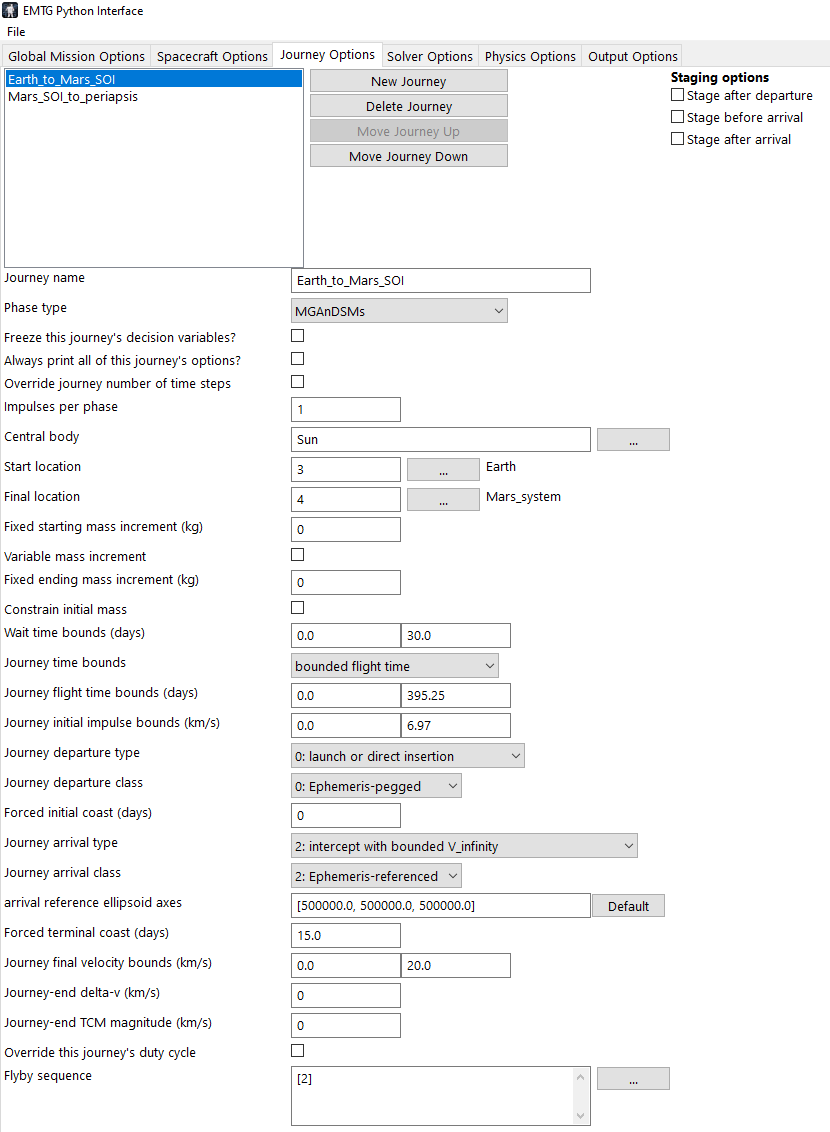
\includegraphics[width=0.9\linewidth]{Journey_Boundaries_earth_to_mars_soi_journey_options.png}}
	\caption{\label{fig:earth_to_mars_soi_options}Earth to Mars \ac{SOI} Journey.}
\end{figure}


\noindent Create a new Journey by clicking the ``New Journey'' button. Use the ``Move Journey Up/Down'' buttons to move the new' Journey below the one from Earth to Mars \ac{SOI}. Make the following additional changes as shown in Figure \ref{fig:mars_soi_to_periapsis_options}:

\begin{itemize}
	\item \textbf{Journey name:} ``Mars\_SOI\_to\_periapsis''
	\item \textbf{Phase type:} ``Coast phase''
	\begin{itemize}
		\item You don’t want to do any maneuvers between crossing the Mars \ac{SOI} until the capture orbit.
	\end{itemize}
	\item \textbf{Wait time bounds (days):} ``0'' to ``0''
	\begin{itemize}
		\item You require epoch continuity at the departure Boundary of this journey.
	\end{itemize}
	\item \textbf{Central body:} ``\texttt{Mars.emtg\_universe}''
	\begin{itemize}
		\item You select the Mars Universe file rather than the Sun Universe file because this Journey takes place within the Mars \ac{SOI}.
	\end{itemize}
	\item \textbf{Journey departure type:} ``2: free direct departure''
	\begin{itemize}
		\item This means that there is no maneuver at the journey departure Boundary.
	\end{itemize}
	\item \textbf{Journey departure class:} ``1: Free point''
	\begin{itemize}
		\item This setting means \ac{EMTG} is free to move the departure Boundary of this Journey around as necessary. The ``Ephemeris-referenced'' setting in the previous Journey will ensure the Boundary is on the Mars \ac{SOI}. The combination of ``Free direct departure'' from a ``Free point'' effectively means that you are constraining the Journey departure boundary state to be equal to the arrival boundary state of the previous Journey (full state continuity).
	\end{itemize}
	\item \textbf{Journey arrival type:} ``1: rendezvous (with chemical maneuver)''
	\begin{itemize}
		\item This will be the orbit insertion burn.
	\end{itemize}
	\item \textbf{Journey arrival class:} ``1: Free point''
	\item \textbf{Journey final impulse bounds:} ``0'' to ``100.0'' km/s
	\begin{itemize}
		\item You are not limiting this maneuver, so you just set an arbitrarily high upper bound.
	\end{itemize}
	\item \textbf{Print a target spec line for free point arrival:} ``On''
	\begin{itemize}
		\item This is so you can see the maneuver in the output files.
	\end{itemize}
	\item \textbf{Journey elements state representation:} `` 3: COE''
	\begin{itemize}
		\item Specifies that you want to use classical orbital elements to define the Mars orbit. 
	\end{itemize}
	\item \textbf{Journey elements frame:} ``0: \acs{ICRF}''
\end{itemize}

\noindent Now, since you are using a free point arrival, a range of acceptable arrival orbit elements can be specified. Each orbit element can be “fixed” at a particular value or allowed to vary within some bounds. You will specify a near-polar, elliptical arrival orbit which might be a good choice for a Mars orbital science mission. (Remember that polar here is with respect to \acs{ICRF} because of the arrival elements frame choice!) Set the arrival elements according to Table \ref{tab:journey_arrival_elements}.

\begin{table}[H]
	\begin{small}
		\begin{tabularx}{\linewidth} { >{\centering\arraybackslash} X >{\centering\arraybackslash} X >{\centering\arraybackslash}X >{\centering\arraybackslash}X  >{\centering\arraybackslash}X   }
			\hline
			Element & Vary & Value & Lower Bound & Upper Bound \\
			\hline 
			SMA (km) & Unchecked & 20000.0 & N/A & N/A \\ 
			ECC & Unchecked & 0.7 & N/A & N/A \\ 
			INC (degrees) & Checked & N/A & 80 & 90 \\
			RAAN (degrees) & Checked & N/A & -360 & 360 \\
			AOP (degrees) & Checked & N/A & -360 & 360 \\
			TA (degrees) & Unchecked & 0.0 & N/A & N/A \\
 			\hline
		\end{tabularx}
	\end{small}
	\caption{\label{tab:journey_arrival_elements}Journey Arrival Elements.}
\end{table}

\begin{figure}[H]
	\centering
	\fbox{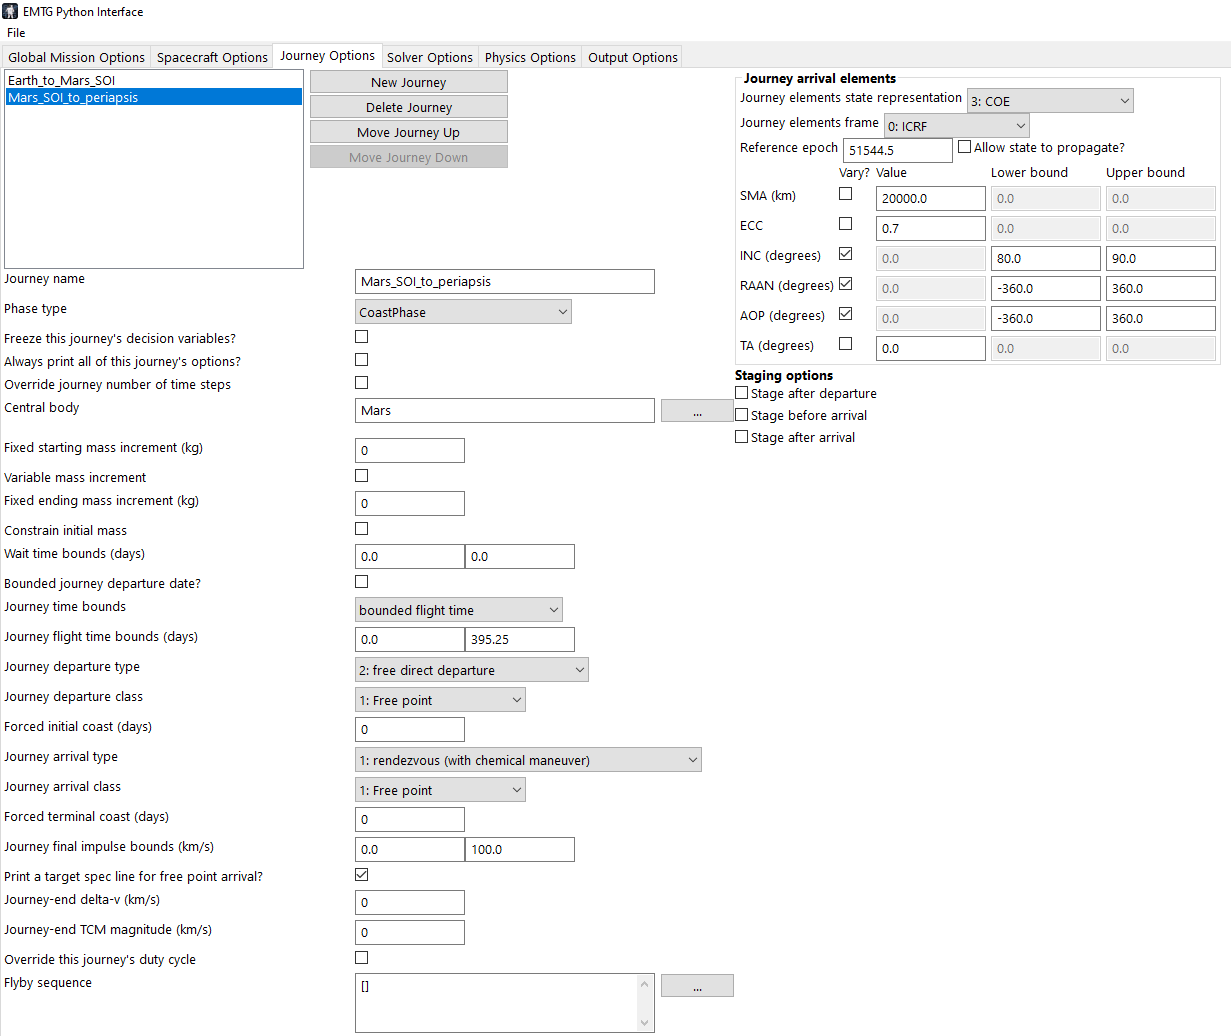
\includegraphics[width=\linewidth]{Journey_Boundaries_mars_soi_to_periapsis_journey_options.png}}
	\caption{\label{fig:mars_soi_to_periapsis_options}Mars \ac{SOI} to Periapsis Journey.}
\end{figure}


%%%%%%%%%%%%%%%%%%%%%
\section{Run and Post-process}
\label{sec:run_and_post_process_jb}
%%%%%%%%%%%%%%%%%%%%%

These are all the required changes. Select “File-\textgreater Run” (Ctrl+r), saving the file as \texttt{EVM\_freepoint.e mtgopt}. If \ac{EMTG} does not find any feasible solutions, change the run time on the ``Solver Options'' tab to 180 seconds or higher (adjusting the ``\acs{MBH} Pareto distribution alpha'' to 1.3 may also help) and try again. EVM\_freepoint is a more difficult problem for \ac{EMTG} to solve than EVM. There are more decision variables and constraints, and the problem is more sensitive. This demonstrates why you usually begin with ephemeris-pegged boundaries instead of ephemeris-referenced or free-point boundaries when designing interplanetary trajectories.

\noindent Open the \texttt{EVM\_freepoint.emtg} solution file in a text editor and note that there are two sections, one for each Journey. In the ``Mars\_SOI\_to\_periapsis'' section, Journey 1 (\ac{EMTG} is starts numbeing at 0), note that the central body is set to Mars. The rows below contain the points defining this Journey, including the cartesian, Mars-centered, \acs{ICRF} states. Check that the magnitude of initial position of the spacecraft (Journey 1, first row, columns X, Y, and Z) is at the \ac{SOI} radius set in the Journey Options tab. The last row in this Journey specifies the Mars orbit after performing the insertion burn. Try converting this cartesian state into COE using \ac{GMAT} or another tool to verify for yourself the correct arrival orbit was reached. Figure \ref{fig:orbit_in_GMAT} shows an example solution visualized using \ac{GMAT}.

\noindent This ends the tutorial on Journey Boundaries. You now know how to specify boundary states in \ac{EMTG} other than those on an ephemeris body. You will revisit this topic when realistic flybys are created in a later tutorial.

\begin{figure}[H]
	\centering
	\fbox{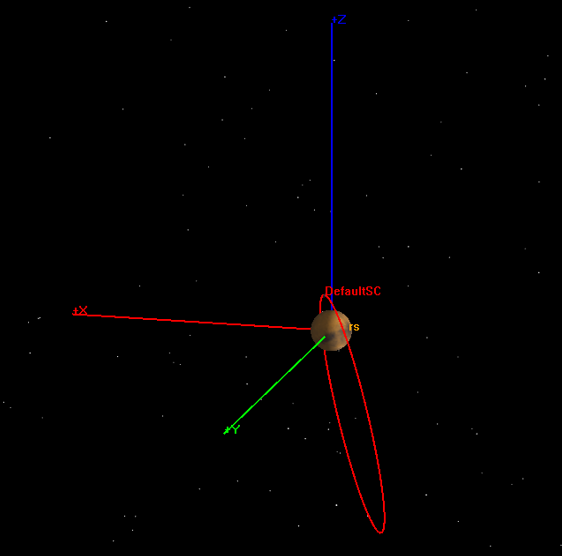
\includegraphics[width=\linewidth]{Journey_Boundaries_Mars_orbit_in_GMAT.png}}
	\caption{\label{fig:orbit_in_GMAT}Mars Orbit Visualized with \ac{GMAT} (Mars \acs{ICRF}).}
\end{figure}


\end{document}